\subsection{Sequence diagram}

\begin{figure}[h]
\centering
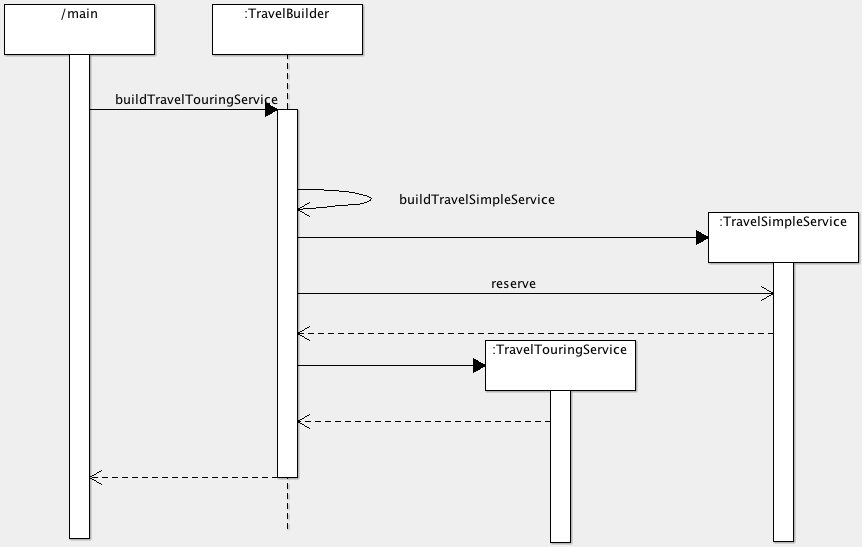
\includegraphics[width=16cm]{project/images/sequence.png}
\caption{Sequence diagram}
\end{figure}

Making a reservation of a touring service have several steps :
\begin{itemize}
\item Main class will make call to method \textit{buildTravelTouringService} of the class \textit{TravelBuilder}
\item TravelBuilder call its own's method \textit{buildTravelSimpleService} 
\item The method \textit{buildTravelSimpleService} create an instance of class \textit{TravelSimpleService}, and use this instance to make a function-call \textit{reserve}
\item The instance created is now used to create an instance of class \textit{TravelTouringService}, and return this new instance to the main class
\end{itemize}